\documentclass{article}
\usepackage{amsmath}
\usepackage{bm}
\usepackage{graphicx}


\title{FLCKS Restaurant Booking System Architecture Document }


\author{
	Christopher Mashele:\\
	\and
	732475\\
	}
\begin{document}

\begin{titlepage}
	
		\hspace{0.5cm}
		\huge
		\center
		\textbf{COMS3008:\\ Software Design}\\

		\vspace*{1cm}
		\Large
		\hspace{2cm}
		\center
		\textbf{FLCKS Restaurant Booking System Architecture Document}\\\\\\
		\vspace*{2cm}
		\normalsize
		\hspace{2.5cm}
		%\textbf{22 July 2016 14h00}

		\textbf{\underline{Team Members}}\\

		\textbf{Mthulisi Leslie Zimba:\hfill570937}

		\textbf{Kgopotso Dilebo:\hfill 715636}

		\textbf{Lethabo Nkabinde:\hfill 722211}

		\textbf{Christopher Mashele:\hfill 732475}
		
		\textbf{Fortune Ndlovu:\hfill 731603}

		
		\vspace{2cm}
		\normalsize
		\hspace{4cm}
		\centre
		
\includegraphics[scale=0.3]{logo}\\
		\hspace{3cm} School of Computer Science and Applied Mathematics\\
		\hspace{3cm}University of the Witwatersrand\\
		\hspace{3cm} South Africa\\
		\hspace{3cm} 5 September 2016 \\
	
\end{titlepage}

\tableofcontents
\pagebreak
\section{\underline{Software Architecture}}
\subsection{Introduction}\\
The following document  pertains to, or describes the architecture of a mobile restaurant booking system application created by FLCKZ,  which works as a booking system for restaurants . The application gives you access to restaurant menus, allows one to book tables and order meals,also check table availability and also rate/share about the service received from the restaurant.\\
\paragraph*{Note}
Certain topics will be discussed at different levels of the Architecture, being relevant to different parties, details to which parties are applicable will be clearly stated.\\\\ The system works on android devices and is downloadable via the Google Play Store on your mobile device.\\


\subsection{References}
Here a list of references used in the creation of this Architecture Document:\\\\
1. D. Garlan & M. Shaw, “An Introduction to Software Architecture,” Advances in Software
Engineering and Knowledge Engineering, Vol. 1, World Scientific Publishing Co. (1993).
2. D. E. Perry & A. L. Wolf, “Foundations for the Study of Software Architecture,” ACM Software
Engineering Notes, 17, 4, October 1992, 40-52.
3. Ph. Kruchten & Ch. Thompson, “An Object-Oriented, Distributed Architecture for Large Scale Ada
Systems,” Proceedings of the TRI-Ada ’94 Conference, Baltimore, November 6-11, 1994, ACM,
p.262-271.
4. G. Booch: Object-Oriented Analysis and Design with Applications, 2nd. edition, Benjamin-Cummings
Pub. Co., Redwood City, California, 1993, 589p.
5. K. P. Birman, and R. Van Renesse, Reliable Distributed Computing with the Isis Toolkit, IEEE
Computer Society Press, Los Alamitos CA, 1994.
6. K. Rubin & A. Goldberg, “Object Behavior Analysis,” CACM, 35, 9 (Sept. 1992) 48-62
7. B. I. Witt, F. T. Baker and E. W. Merritt, Software Architecture and Design—Principles, Models, and
Methods, Van Nostrand Reinhold, New-York (1994) 324p.
8. D. Garlan (ed.), Proceedings of the First Internal Workshop on Architectures for Software Systems,
CMU-CS-TR-95-151, CMU, Pittsburgh, 1995.
 
\pagebreak
\section{\underline{Architectural goals and concerns}}
This document aims to show how our application will work and to form a blueprint which will enable one to navigate and explore easily through the Application to give one a better idea as to what our Application does.\\\\

\subsection{Software Decisions}
The System that we are creating is intended to perform well in an ever-changing environment because it is intended on being used on a daily basis, keeping in mind that it also needs to be very secure and thus we wouldn't want any data to be leaked/published, because confidential information will be dealt with. We also want a high performing application. We expect the application to be accessed by a large number of people and thus would like to be able to upgrade/ scale up if needs be in order to accommodate large volumes of users in the future.\\\\ With that in mind we have decided to use the event-driven architectural style because it performs well in the key factors required for the application. We will be using the Mediator Topology in the creation of the Application due to a number of different factors, which will be explained throughout the document.\\\\ Our Application will have two main users, namely the Client and the Administrator, thus we found it fitting that since the Administrator will be at work most of the time, that they should access their Administrative privileges using their office computer. Thus no cost will be put to the company in terms of mapping the software to hardware, they just use their current Office PC.\\ The Client on the other Hand will only be able to access the system via an android device. This decision was made due to recent statistics that show the ever increasing number of android devices available and the number of people who use android devices today.\\\\ Depicted is the Architecture Decision diagram, where the black blocks represent the type of functionality and the box below depicts the domain to which the functionality will be accessed.\\\\

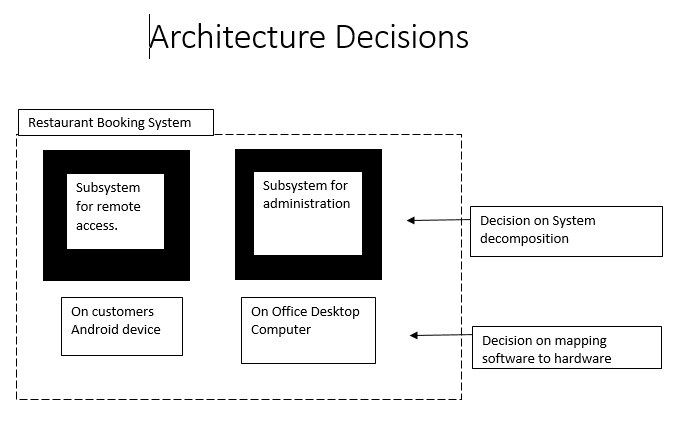
\includegraphics[scale=0.5]{Decisions}\\
Figure 1: Decision Diagram
%\section{\underline{Stakeholders}}
%\section{\underline{Logical Architecture}}
%\section{\underline{Process Architecture}}
\pagebreak
\section{\underline{Development Architecture Style}}
In this section we will discuss the type of Architecture Style that our Booking System will abide to.\\
\subsection{Architecture Decomposition}
Diagrams in this section give a basic Architectural overview of an Application designed using the Mediator Event-driven design Topology. This could, in essence, be viewed as the blueprint design of our Application.\\\\ The Application Can be decomposed into multiple events that occur at any given state of the application, these events take the form of signals (clicks, scrolls etc) which require some process/channel to be triggered. This is depicted nicely in the following diagram.\\\\


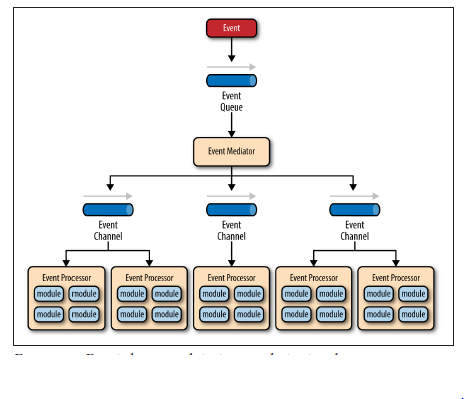
\includegraphics[scale=0.6]{Capture}\\
Figure 2: Architecture Decomposition

\subsection{Event-Driven Approach}
There are four main types of architecture components within the
mediator topology: event queues, an event mediator, event channels,
and event processors. The event flow starts with a client sending an
event to an event queue, which is used to transport the event to the
event mediator. The event mediator receives the initial event and
orchestrates that event by sending additional asynchronous events
to event channels to execute each step of the process. Event processors,
which listen on the event channels, receive the event from the
event mediator and execute specific business logic to process the
event.\\

\paragraph*{Note:}
The following is intended for the more technically inclined and involves high levels of jargon.\\ We are intending on having 10's of event queue's in our Architecture consisting of message queues and web service endpoints.\\\\ The initial event patterns will take the form of clicks and scrolls on the GUI of the system and the processing events will be in forms of database operations and changes. The event-mediator that we will be using is in the form of PHP scripts which are responsible for orchestrating the steps contained within the initial event. For each step in the initial event, the event-mediator(PHP scripts) sends out a specific processing event to an event channel, which is then received and processed by the event processor.\\\\ Event channels will be in the form of PHP commands which come directly from the event-mediator to pass specific processing events related to the initial processing command, message topics will be used.
We will be using a Local host server as our event processor and it will have tables pertaining of all the required fields necessary to satisfy all business logic and thus will be able to satisfy any processing event. It will be a self-contained, independent on line server that will be the backbone of business relations to the Application. The granularity of the event processor will range from very basic events (booking a table) to more complicated ones (such as ordering multiple meals).\\\\

\pagebreak
\section{\underline{Physical Architecture}}
\subsection{{System Summary}}
At a very high level of the system the application will be transitioning through a series of states (pages) where the events will trigger the event-mediator and that data will be visible to the event processor.\\\\ To really get an idea of how this all will unfold, the best way to depict it will be a physical view of the application. Figure 3 represents an event that we will take into consideration. Consider a logged in client that wants to be able to use the application, he will go to the home page (Figure 3)\\\\\

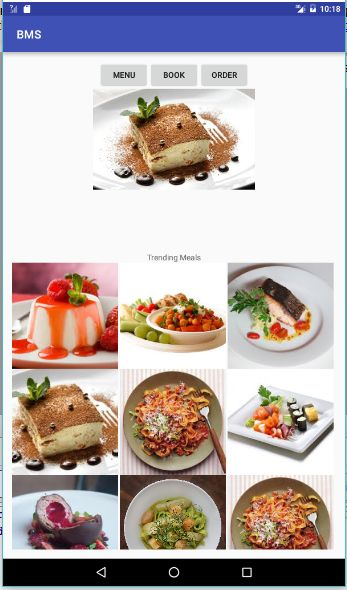
\includegraphics[scale=0.4]{Menu}\\  
Figure 3 : Home Page\\\\ Here, the client will be given various options (either book, order, view menu etc..), let's say that he decides to book a table (given that this is a Booking system). Logically, the view he is presented with should in truth change.. Thus an event occurs and a signal is taken by the event-mediator (This time just simple .java & .xml code), the event-mediator then deploys an event channel signalling that another state should be produced to accommodate that and another event. Resulting in another screen being displayed namely, Yep you guessed it, the Booking page. Figure 4 displays the booking page.\\
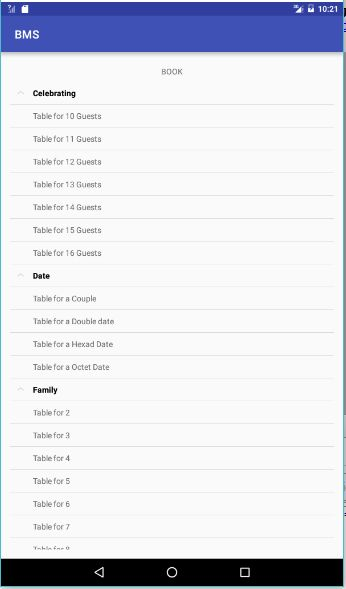
\includegraphics[scale=0.4]{Book}\\ 
Figure 4: Booking page\\\\ Here we see again that there are many "events" that could take place, namely choosing the table that the client would like to book(depending on size and occasion). Now that signal/ event is sent to the event-mediator, this time, being the PHP scripts that should communicate to the local host on line server. That signal then changes the database and a signal is sent back to confirm the change. Which is depicted by Figure 5.\\\\
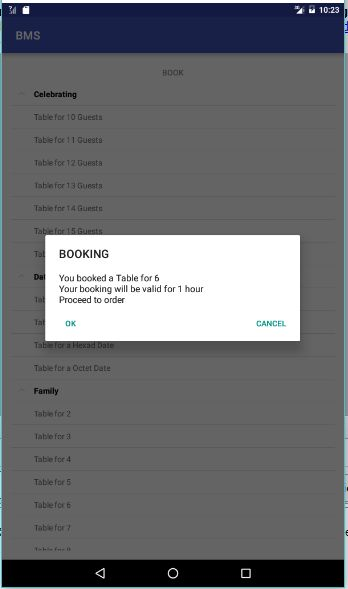
\includegraphics[scale=0.4]{BookConfirm} \\
Figure 5: Booking Confirmation\\\\ Here a signal sent and then you are prompted to order if you are interested.
\pagebreak
\section{\underline{Scenarios}}
\subsection{{Types of Scenarios}}
True there are many different scenarios that could take place, as mentioned in the topic discussed above, and not all can be mentioned in this documentation. But a brief overview of the most basic and common scenarios that will be considered, due to the nature of the system as a whole. Here is a list of the top scenarios that will be fulfilled by the System:
\begin{itemize}
\item Register: This scenario is the first experience you have with the Application, it enables you to create your user profile and adding your details to the local host database system.
\item Login: Once you have a profile, this scenario allows you to access the Application and gives a client the ability to start performing the different tasks given to them by the Application. 
\item Logout: Once you have completed your given tasks, then it allows you to exit your profile and login another profile.
\item View menu: This scenario will be one of the most common because if you dont want to book a table, you can still use this scenario in order to keep up to date with the current meals and specials offered by the restaurant.
\item Book table: This is also a common scenario and was mentioned in detail in the above section.
\item Order meal: This can be done by selecting the meals you fancy in the menu and clicking requesting it by clicking on the order button. 
\end{itemize}
\paragraph{•}
These are some of the functionalities we are working on:
\begin{itemize}
\item Rate service: This will enable you to rate the service you recieved both by the restaurant and the Application in store. More details will revealed as the progress of the Application unfolds.
\item Share experience on social media: Brag to your friends on your experience with the Application and restaurant.
\end{itemize}

\pagebreak
\section{\underline{Size and Performance}}
\subsection{Feedback}

We have, thus far, not done a particular analysis on the design of the software so we cannot  yet conclude how the software will perform and the size required to build it.\\\\ For now though we have created a local host server which will be able to hold a couple of hundred of clients due to financial constraints, but given that we created the system in compliance with the Event-Driven Mediator Topology which gives room for up scaling abilities and we intend on scaling up as the application takes flight.\\\\ Another advantage that we got by using this Architectural style is that it allows a system to perform well since Event processes are independent and are able to be performed in parallel. Our team of programmers(who are clued up in Parallel Computing) intend on using their broad insight in their respective field to ensure that the System performs as optimal as possible.\\\\ Since in truth we are using the Agile methodology in the creation of the system, thus estimations of the performance and size are subject to change depending on the stage of production. 
\pagebreak
\section{\underline{Quality}}
\subsection{{Words From Scrum Master}}

We are implementing rigorous testing techniques for all aspects of the Application and thus we are confident that our Application will be as(if not, more) efficient and competitive as applications available on today's market.
\pagebreak
\section{\underline{Appendices }}
\subsection{{Acronyms and Abbreviations}}
Some Acronyms and Abbreviations used in this document are mentioned below:
\begin{itemize}
\item FLCKZ: Design team name derived from the names of the group Members (Fortune, Lethabo,Chris,Kgopotsho, Mthulisi (Zimba))
\item GUI: Graphic User Interface 

\end{itemize}
\subsection{{Definitions}}
Some Definitions explained:
\begin{itemize}
\item PHP: A server-side scripting language designed for web development.
\item Event-Driven Architecture: An Architecture development design Technique
\item Event-mediator: The event mediator receives the initial event and
orchestrates that event by sending additional asynchronous events
to event channels to execute each step of the process.
\item Event-process: which listen on the event channels, receive the event from the
event mediator and execute specific business logic to process the
event.


\end{itemize}
%\subsection{{Design Principles}}

\end{document}
